\chapter{Aplicación sobre datos}

\section{Cemento, análisis estructural y capacidades predictivas.}
\subsection*{Descripción del dataset}
\noindent El dataset  \cite{Yeh 2007} es un conjunto de datos recogidos de distintos tipos de cementos con distintas densidades, en particular tenemos las siguientes variables:
\begin{table}[h]
\footnotesize
\centering
\begin{tabular}{|l|l|l|l|}
\hline
Nombre & Tipo de dato & Medida & Descripción \\
\hline
Cemento (variable 1) & continuo & kg en una mezcla m3 & Variable predictora \\
Escoria de alto horno (variable 2) & continuo & kg en una mezcla m3 & Variable predictora \\
Ceniza volante (variable 3) & continuo & kg en una mezcla $m^3$ & Variable predictora \\
Agua (variable 4) & continuo & kg en una mezcla $m^3$ & Variable predictora \\
Superplastificante (variable 5) & continuo & kg en una mezcla $m^3$ & Variable predictora \\
Agregado grueso (variable 6) & continuo & kg en una mezcla $m^3$ & Variable predictora \\
Agregado fino (variable 7) & continuo & kg en una mezcla $m^3$ & Variable predictora \\
Edad & continuo & Día (1-365) & Variable predictora \\
Resistencia a la compresión & continuo & MPa & Variable respuesta \\
\hline
\end{tabular}
\caption{Tabla resumen de las variables estudiadas}
\label{tab:Resumen Variables}
\end{table}

\noindent Se recogen de manera esquemática en el cuadro \ref{tab:Resumen Variables}. 


\noindent El tamaño de la muestra es de 1030 observaciones, de las cuales un $70\%$ se separan para realizar el ajuste de los distintos modelos y el $30\%$ restante se utilzará para calcular la capacidad predictiva de los modelos. 

\subsection*{Objetivos}

\noindent Este estudio tiene dos objetivos principales:
\begin{itemize}
\item Detallar y analizar patrones de comportamiento en los cementos en base a las características descritas. 
\item Crear y analizar distintos modelos que permitan la predicción de la resistencia a la compresión. 
\end{itemize}
\subsection*{Metodología}

\noindent Para conseguir el primer objetivo se utilizará el análisis de componentes principales. Con ello, se podrá estudiar la estructura de los datos de manera que se vea que variables afectan en mayor medida a la varianza. 

\noindent Para el otro objetivo se ajustarán   tres modelos distintos. Un modelo de regresión lineal, un árbol de regresión y una red neuronal. Se describirán las cualidades que aporta cada uno de los modelos y se compararán. Es por ello que se separará el conjunto de datos en dos partes una de ajuste y otra de comprobación de las capacidades predictivas. 

\noindent En particular, se utilizará el error cuadrático medio, \emph{MSE}, en cada uno de los modelos, de manera que en el conjunto de entrenamiento servirán como medida de bondad de ajuste y en el conjunto de comprobación para probar sus capacidades predictivas. 

\noindent A nivel técnico, para esta parte se utilizará el lenguaje de programación Python. En particular, se usan las siguientes librerías:
\begin{itemize}
\item \emph{Pandas:} para el tratamiento previo de los datos. 
\item \emph{Scikit-Learn:} usado en el ajuste de los distintos modelos \cite{Scikit-Learn}. 
\item \emph{Numpy:} utilizado en el manejo de las matrices y los vectores
\item \emph{Matplotlib} empleado para la generación de los distintos gráficos \url{https://matplotlib.org/}.
\end{itemize}

\subsection*{Desarrollo y resultados}

\noindent Para empezar, se hace un análisis descriptivo básico de cada una de las variables:
\begin{figure}[h]
  \centering
  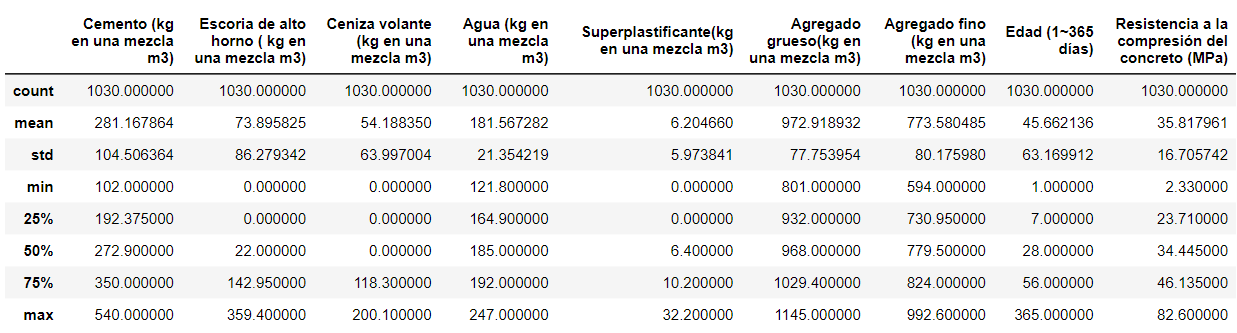
\includegraphics[scale=0.55]{Documentos Extra/Imagenes/Resumen_Basicos.png}
  \caption{Análisis descriptivo de los datos}
  \label{fig:resumen_basicos}
\end{figure}

\noindent En este primer análisis resumido en la figura \ref{fig:resumen_basicos} podemos ver que la media de la fuerza de compresión o resistencia a la compresión tiene una media muestral de $35,82$ MPa, con una desviación estándar de $16,70$ MPa lo cual nos dice que hay una alta dispersión de los datos en este caso. Hay que tener esto en cuenta ya que puede afectar a los errores de los distintos modelos. 

\noindent Hay otras medidas a las que le ocurre lo mismo, es decir, que tienen una alta dispersión como pueden ser las cantidad de superplastificante, la ceniza volante o la escoria de horno. 

\noindent También hay que destacar que al menos un $50\%$ de las observaciones no tiene ceniza volante.  

\noindent Ahora se calculan las componentes principales utilizando la matriz estandarizada. Después de aplicar este proceso, obtenemos la proporción acumulada de la varianza explicada en cada una de las componentes:
\begin{equation*}
[0.25, 0.47, 0.63, 0.74, 0.85, 0.95, 0.98, 1.  , 1.  ]
\end{equation*}


%\begin{figure}[h]
%  \centering
%  \includegraphics[scale=0.5]{Documentos Extra/Imagenes/Gráfico_varianza_explicada.png}
%  \caption{Varianza acumulada frente al número de componentes principales}
%  \label{ratio_varianzas}
%\end{figure}

\noindent En particular, cuando tomamos las 3 primeras componentes principales estas representan un $62.5$\% de la variabilidad total, en particular esas componentes representan una variabilidad del  $25\%, 22\%, 16\%$ respectivamente. Podríamos llegar a a un $85\%$ si cogiésemos las 5 primeras. En nuestro caso, nos quedaremos con 3 para poder representar los datos en un espacio de dimensión reducida. 

\noindent Los coeficientes de las componentes principales obtenidos son los siguientes:

\begin{equation}
Z_1
\end{equation}
\begin{equation}
Z_2
\end{equation}
\begin{equation}
Z_3
\end{equation}

\noindent Al haber trabajado con la matriz estandarizada, estas cargas también representan la correlación de cada una de las variables con la componente en cuestión. 

\noindent Aquellas variables que tienen una carga en las componentes principales mayor que $0.5$ en valor absoluto tienen una relación importante con las componentes. En cambio, todas aquellas cercanas al $0$ no tienen una relación menor con la componente. 

\noindent Se ajustan 3 modelos distintos, un modelo lineal, un árbol de regresión, y una red neuronal. 

\noindent Las características de los modelos y de los procesos de ajuste son los siguientes:

\noindent El modelo lineal es ajustado  obteniéndose un mínimo de error cuadrático de $106.14$ en el conjunto de entrenamiento.  Mientras que en el conjunto de comprobación se obtiene un error cuadrático medio de $108,21$. Además aunque no se pueda usar en el resto de modelos se obtiene en este caso un coeficiente de determinación $R^2$ de $0,62$ en el conjunto de ajuste. Por tanto, no tiene un buen nivel predictivo. 

\noindent El árbol de decisión utiliza el criterio \emph{CART} de Breiman, ya que es el implementado por defecto en la librería \emph{Scikit-Learn} de Python \cite{Breiman 1984}. Este modelo proporciona un error cuadrático medio de  $108.22$ sobre el conjunto de ajuste mientras que sobre el conjunto de testeo proporciona un error cuadrático de $57.55$, lo que implica que tiene una mejor capacidad predictiva que el modelo lineal pero aún así deja que desear. 

\noindent En la red neuronal se ha elegido un modelo simple con dos capas, la primera con 13 neuronas con una función de activación lineal rectificada, en cambio, la otra capa contiene únicamente una neurona con una función lineal. En este caso el ajuste de la red neuronal obtiene un error cuadrático medio de $MSE=46.56$ en el ajuste y un $MSE=47.54$ en el conjunto de prueba, en principio, tenemos un modelo que comete menos error en el conjunto de prueba. 

\noindent Hay que destacar que ninguno de los modelos ha incurrido en problemas de sobreajuste, es decir, no se ha tenido casos en los que el valor del error medio en el conjunto de ajuste sea mucho menor que en el conjunto de prueba. 

\noindent Una vez ajustados los modelos, se pueden tomar los valores predichos para los datos de prueba y graficarlos frente a los valores reales, en cada caso tendremos los puntos en azul y la recta roja representaría los puntos los cuales su predicción es igual al valor real. 

\begin{figure}[ht]
  \centering
  \begin{minipage}{0.32\textwidth}
   
    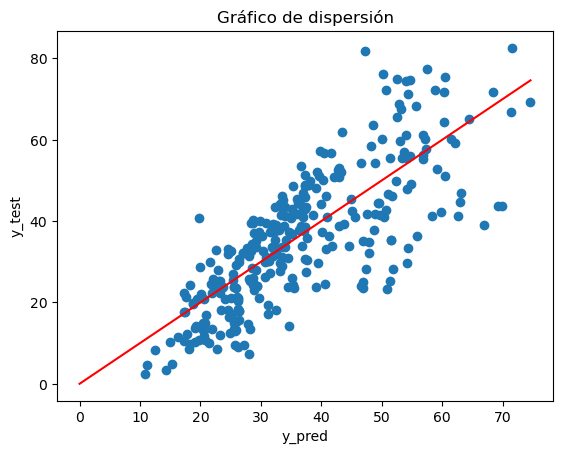
\includegraphics[width=\textwidth]{Documentos Extra/Imagenes/Datos PruebasRegresionLineal.png}
    \caption{Regresión Lineal}
    \label{fig:regresion_lineal}
  \end{minipage}
  \hfill
  \begin{minipage}{0.32\textwidth}
 
    \includegraphics[width=\textwidth]{Documentos Extra/Imagenes/Datos PruebasÁrbolesRegresion.png}
    \caption{Árbol de Regresión}
    \label{fig:regression_tree}
  \end{minipage}
  \begin{minipage}{0.32\textwidth}
    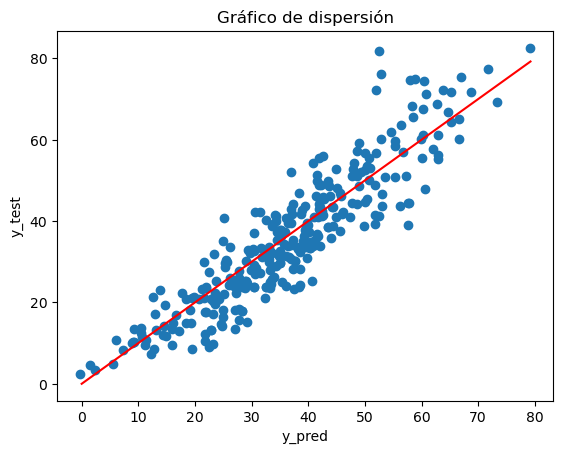
\includegraphics[width=\textwidth]{Documentos Extra/Imagenes/Datos PruebasRedNeuronal.png}
    \caption{Red Neuronal}
    \label{fig:red_neuronal}
  \end{minipage}
 \end{figure}

\noindent Se puede ver que en el caso del modelo lineal \ref{fig:regresion_lineal} los puntos son más lejanos de la recta. Por tanto, tenemos que el primer caso en principio tendrá peores predicciones. 

\noindent En resumen, obtenemos los siguientes resultados:

\begin{table}[ht]
\centering
\begin{tabular}{|l|c|c|c|}
\hline
 & Modelo Lineal & Árbol de Regresión &  Red Neuronal \\
\hline
Conjunto Ajuste &  $106.14$  &  $108.22$& $46.56$\\
Conjunto de Prueba & $108,21$   & $57.55$ &  $47.54$ \\
\hline
\end{tabular}
\caption{Errores cuadráticos medios en cada conjunto}
\label{tab:tabla_ejemplo}
\end{table}

\noindent En conclusión, los modelos en este caso no han conseguido el objetivo principal que era diseñar un modelo con buenas capacidades predictivas. Concretamente, ha sido el modelo de la red neuronal el que mejores resultados ha obtenido, pero su alta complejidad lastra su interpretabilidad. En cambio, el árbol de regresión obtiene en el proceso de prueba resultados similares y además con una fácil interpretación debido a que se puede representar como un diagrama de árbol. 

